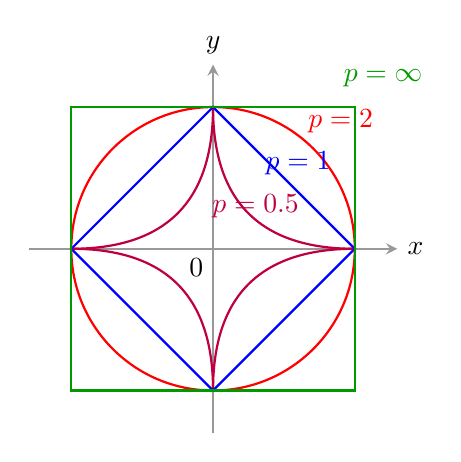
\begin{tikzpicture}[scale=1.8]
            % Axes
            \draw[->,>=stealth,gray!80,thick] (-1.3,0) -- (1.3,0) node[right,text=black] {$x$};
            \draw[->,>=stealth,gray!80,thick] (0,-1.3) -- (0,1.3) node[above,text=black] {$y$};
            
            % p = 0.5 (Non-convex, astroid-like)
            \draw[domain=0:90, samples=100, color=purple, thick] plot ({cos(\x)*cos(\x)*cos(\x)*cos(\x)}, {sin(\x)*sin(\x)*sin(\x)*sin(\x)});
            \draw[domain=90:180, samples=100, color=purple, thick] plot ({-cos(\x)*cos(\x)*cos(\x)*cos(\x)}, {sin(\x)*sin(\x)*sin(\x)*sin(\x)});
            \draw[domain=180:270, samples=100, color=purple, thick] plot ({-cos(\x)*cos(\x)*cos(\x)*cos(\x)}, {-sin(\x)*sin(\x)*sin(\x)*sin(\x)});
            \draw[domain=270:360, samples=100, color=purple, thick] plot ({cos(\x)*cos(\x)*cos(\x)*cos(\x)}, {-sin(\x)*sin(\x)*sin(\x)*sin(\x)});

            % p = 1 (Diamond)
            \draw[thick, blue] (1,0) -- (0,1) -- (-1,0) -- (0,-1) -- cycle;
            
            % p = 2 (Circle)
            \draw[thick, red] (0,0) circle (1);
            
            % p = infinity (Square)
            \draw[thick, green!60!black] (-1,-1) rectangle (1,1);
            
            % Labels
            \node[purple] at (0.3,0.3) {$p=0.5$};
            \node[blue] at (0.6,0.6) {$p=1$};
            \node[red] at (0.9,0.9) {$p=2$};
            \node[green!60!black] at (1.2,1.2) {$p=\infty$};
            \node[below left] at (0,0) {$0$};
        \end{tikzpicture}